%%
%% Copyright 2007, 2008, 2009 Elsevier Ltd
%%
%% This file is part of the 'Elsarticle Bundle'.
%% ---------------------------------------------
%%
%% It may be distributed under the conditions of the LaTeX Project Public
%% License, either version 1.2 of this license or (at your option) any
%% later version.  The latest version of this license is in
%%    http://www.latex-project.org/lppl.txt
%% and version 1.2 or later is part of all distributions of LaTeX
%% version 1999/12/01 or later.
%%
%% The list of all files belonging to the 'Elsarticle Bundle' is
%% given in the file `manifest.txt'.
%%

%% Template article for Elsevier's document class `elsarticle'
%% with numbered style bibliographic references
%% SP 2008/03/01
%%
%%
%%
%% $Id: elsarticle-template-num.tex 4 2009-10-24 08:22:58Z rishi $
%%
%%
\documentclass[review ,12pt,3p]{elsarticle}

%% Use the option review to obtain double line spacing
%% \documentclass[preprint,review,12pt]{elsarticle}

%% Use the options 1p,twocolumn; 3p; 3p,twocolumn; 5p; or 5p,twocolumn
%% for a journal layout:
%% \documentclass[final,1p,times]{elsarticle}
%% \documentclass[final,1p,times,twocolumn]{elsarticle}
%% \documentclass[final,3p,times]{elsarticle}
%% \documentclass[final,3p,times,twocolumn]{elsarticle}
%% \documentclass[final,5p,times]{elsarticle}
%% \documentclass[final,5p,times,twocolumn]{elsarticle}

%% if you use PostScript figures in your article
%% use the graphics package for simple commands
%% \usepackage{graphics}
%% or use the graphicx package for more complicated commands
%% \usepackage{graphicx}
%% or use the epsfig package if you prefer to use the old commands
%% \usepackage{epsfig}

%% The amssymb package provides various useful mathematical symbols
\usepackage{amssymb}
%% The amsthm package provides extended theorem environments
%% \usepackage{amsthm}

%% The lineno packages adds line numbers. Start line numbering with
%% \begin{linenumbers}, end it with \end{linenumbers}. Or switch it on
%% for the whole article with \linenumbers after \end{frontmatter}.
%% \usepackage{lineno}

%% natbib.sty is loaded by default. However, natbib options can be
%% provided with \biboptions{...} command. Following options are
%% valid:

%%   round  -  round parentheses are used (default)
%%   square -  square brackets are used   [option]
%%   curly  -  curly braces are used      {option}
%%   angle  -  angle brackets are used    <option>
%%   semicolon  -  multiple citations separated by semi-colon
%%   colon  - same as semicolon, an earlier confusion
%%   comma  -  separated by comma
%%   numbers-  selects numerical citations
%%   super  -  numerical citations as superscripts
%%   sort   -  sorts multiple citations according to order in ref. list
%%   sort&compress   -  like sort, but also compresses numerical citations
%%   compress - compresses without sorting
%%
%% \biboptions{comma,round}

% \biboptions{}

\usepackage{multirow}
\usepackage{framed}
\usepackage{amsmath}



\journal{Expert Systems with Applications}

\begin{document}

\begin{frontmatter}

\title{R\'esuMatcher: A Personalized R\'esum\'e-Job Matching System}
\tnotetext[label0]{This is only an example}


\author[label1,label2]{Author One\corref{cor1}\fnref{label3}}
\address[label1]{Address One}
\address[label2]{Address Two\fnref{label4}}

\cortext[cor1]{I am corresponding author}
\fntext[label3]{I also want to inform about\ldots}
\fntext[label4]{Small city}

\ead{author.one@mail.com}
\ead[url]{author-one-homepage.com}

\author[label5]{Author Two}
\address[label5]{Some University}
\ead{author.two@mail.com}

\author[label1,label5]{Author Three}
\ead{author.three@mail.com}

\begin{abstract}
Today, online recruiting web sites such as Monster and Indeed.com have become one of the main channels for people to find jobs. These web platforms have provided their services for more than ten years, and have saved a lot of time and money for both job seekers and organizations who want to hire people. However, traditional information retrieval techniques may not be appropriate for users. The reason is because the number of results returned to a job seeker may be huge, so job seekers are required to spend a significant amount of time reading and reviewing their options. One popular approach to resolve this difficulty for users are recommender systems, which is a technology that has been studied for a long time.

In this thesis we have made an effort to propose a personalized job-r\'esum\'e matching system, which could help job seekers to find appropriate jobs more easily. We create a finite state transducer based information extraction library to extract models from r\'esum\'es and job descriptions. We devised a new statistical-based ontology similarity measure to compare the r\'esum\'e models and the job models. Since the most appropriate jobs will be returned first, the users of the system may get a better result than current job finding web sites. To evaluate the system, we computed Normalized Discounted Cumulative Gain (NDCG) and precision@k of our system, and compared to three other existing models as well as the live result from Indeed.com.
\end{abstract}

\begin{keyword}
%% keywords here, in the form: keyword \sep keyword
Recommender system \sep Ontology  \sep R\'esum\'e \sep Job Description
%% MSC codes here, in the form: \MSC code \sep code
%% or \MSC[2008] code \sep code (2000 is the default)
\end{keyword}

\end{frontmatter}

%%
%% Start line numbering here if you want
%%
% \linenumbers

%% main text

\section{Introduction}
\label{sec1}

Currently one of the main channels for job seekers is online job finding web sites, like Indeed or  Monster etc., that make the job finding process easier and decrease the recruitment time. But most such web sites only allow users to use keywords to search the jobs, which makes job searching tedious and blind task. For example, I used keyword ``Java'' to search jobs with location restriction Mountain View, CA on the job searching site indeed.com, the web site returned about 7,000 jobs (Figure~\ref{fig:Indeed}). The number of results of job searching is huge but not well ranked, so the job seeker has to review every job description. Since no one has enough time to read all the jobs in the searching result, the actual quality of job searching service is low. This is a classic problem of information overflow.

\begin{figure}[htbp]
  \centering
  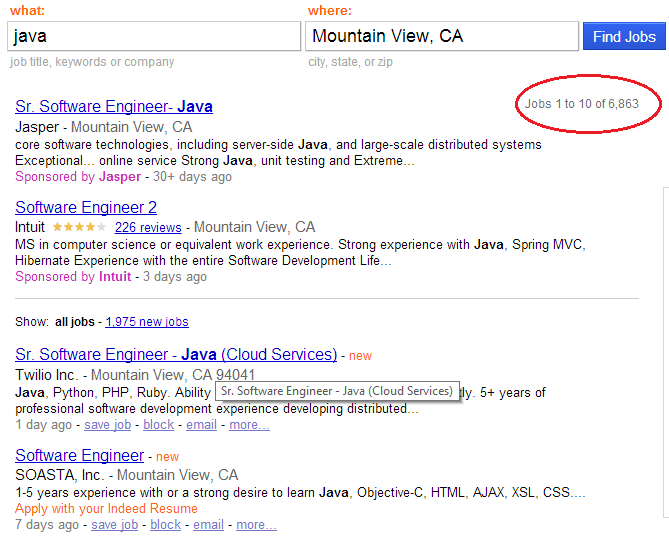
\includegraphics[scale=0.6]{images/indeed1.png}
  \caption{Search result of Indeed.com}
  \label{fig:Indeed}
\end{figure}

The reason for such a result is because current job searching web sites use the same information retrieval technology like ``Inverted index'' \cite{zobel2006inverted} as the common search engines, which just use keywords to map all the stored documents. Modern search engines all have some ranking algorithms to sort the search result, like page rank \cite{page1999pagerank}, so the top results always be the most related ones. But such algorithms are unavailable to the job search systems, because the criteria  of how to rank the job searching result is very personalized. A great job opening for one job seeker maybe looks not good to the other, because the goodness of a job to a specular job seeker is heavily depend on his personal background, like his education or professional experience etc.

Since the people's r\'esum\'es contain the most important background information, we believe the content of the r\'esum\'e could be used to rank the job openings. In this paper, we created a web system which uses the r\'esum\'es of job seekers to find the jobs that match their profiles best. The main idea is to calculate the similarity between the r\'esum\'e model and job models, which should be generated from r\'esum\'es and job descriptions. We want to transfer the job searching task from key word searching to candidate model matching. The matching result should be sorted by the matching score, higher matching score means a better matching. The matching algorithm does not only help job seekers to find the appropriate jobs, but also offers priority to them~\cite{gueutal2006brave}.  The job with higher matching score means the job is more appropriate to the job seeker, and if he applies to the job, the chance of getting the interview will be higher as well.

We make the following contributions in this work:

\begin{enumerate}
    \item  We proposed a r\'esum\'e - job matching system.
    \item  We proposed a finite state transducer based matching tool to extract information from unstructured data source, which is a lightweight and flexible library, and can be extended in very easy ways.
    \item  We proposed a semi-automatic approach, which can collect technical terms from hr data sources, and by which we created a domain specific ontology for recruitment.
    \item  We proposed statistical-based ontology similarity measure, which can measure the similarities between technical terms .
\end{enumerate}

The subsequent sections are organized as follows: Section 2 describes what has been done in terms of prior work. Section 3 gives a overview of our system, R\'esuMatcher, the Personalized R\'esum\'e-Job Matching System. In section 4 we explains details of how we resolve the problems of information extraction. In section 5, we explains the model similarity calculation. Section 6 describes how to construct the Ontology and how to calculate the similarities in ontology. Section 7 describe the evaluation result of our system. Finally Section 8 shows the conclusions and future line of work.

\section{Related Works}
\label{sec1}

Some scholars found that current boolean search and filtering techniques cannot satisfy the complexity of candidate-job matching requirement~\cite{malinowski2006matching}. They hope the system can understand the job requirement, determine which requirements are mandatory and which are optional, but preferable. So they moved to use recommender systems technique to address the problem of information overflow. Recommender systems are broadly accepted in various areas to suggest products, services, and information items to latent customers.

\subsection{Recommender System}
\label{subsec1}

Job searching, which has been the focus of some commercial job finding web sites and research papers is not a new topic in information retrieval. Usually scholars called them Job Recommender Systems (JRS), because most of them used technologies from recommender systems. Wei et al. classified Recommender Systems into four categories~\cite{wei2007survey}:

\begin{enumerate}
    \item Content-based Recommendation (CBR). The principle of a content-based recommendation is to suggest items that have similar content information to the corresponding users, like Prospect \cite{singh2010prospect}.

    \item Collaborative Filtering Recommendation (CFR). Collaborative filtering recommendation finds similar  users  who have  the same taste with the target user and recommends items based on what the similar users, like CASPER~\cite{rafter2000personalised}.

    \item Knowledge-based Recommendation (KBR). In the knowledge-based recommendation, rules and patterns obtained from the functional knowledge of how a specific item  meets the requirement of a particular user, are used for recommending items, like  Proactive~\cite{lee2007fighting}.

    \item Hybrid recommender systems combine two or more recommendation techniques to gain better performance, and overcome the drawbacks of any individual one. Usually, collaborative filtering is combined with some other technique in an attempt to avoid the ramp-up problem.

\end{enumerate}

\subsection{Job Recommender System}

Rafter et al. began to use Automated Collaborative Filtering (ACF) in their Job Recommender System, ``CASPER''  \cite{rafter2000personalised}. The system use cluster-based collaborative filtering strategy. The similarity between users are based on how many jobs they both reviewed, or applied. F{\"a}rber et al. \cite{farbr2003automated} presented a recommender system built on a hybrid approach. The system integrate two methods, content-based filtering and collaborative filtering, which tries to overcome the problem of rating data sparsity by leveraging a combined model. In the system, the data source is synthetic resumes. 

\subsection{Information Extraction in Job Recommender System}

Big IT companies met the similar problem of information overflow when they received many resumes for one job opening. The recruiter had to screen the all the applications manually, but this task was also tedious and time consuming. For this reason these companies tried to build systems to help screen the resumes.

Amit et al. in IBM presented a system, ``PROSPECT''~\cite{singh2010prospect}, to aid shortlisting candidates for jobs. The system uses a r\'esum\'e miner to extract the information from r\'esum\'es, which use a conditional random field (CRF) model to segment and label the r\'esum\'es. HP also built a system to solve the similar problem, which is introduced in Gonzalez et al.'s paper~\cite{gonzalez2012adaptive}. The system uses a layered information extraction framework to processing r\'esum\'es. The goal of the systems built by IBM and HP is to help the companies to select good applicants, but cannot help job seekers to find appropriate jobs.

Yu et al.~\cite{yu2005resume} used a cascaded IE framework to get the detailed information from the r\'esum\'es. In the first stage, the Hidden Markov Modeling (HMM) model is used to segment the r\'esum\'e into consecutive blocks. Based on the result, a SVM model is used to obtain the detailed information in the certain block, the information include: name, address, education etc. Celik Duygua and Elci Atilla proposed a Ontology-based R��sum�� Parser (ORP)~\cite{ccelik2013ontology}, which uses ontology to assistant the information extraction process. The system processes a r\'esum\'e in following steps: converting the r\'esum\'e file into plain text, separating the text into some segments, using the ontology knowledge base to find the concepts in the sentences, normalizing all the terms, and classifing the sentences to get the wanted terms.

\subsection{Matching Algorithms in Job Recommender Systems}

Lu et al.~\cite{lu2013recommender} used latent semantic analysis (LSA) to calculate similarities between jobs and candidates, but they only selected two factors ``interest'' and ``education''  to compare candidates. Xing et al.~\cite{yi2007matching} used structured relevance models (SRM) to  match r\'esum\'es and jobs. Drigas et al.\cite{drigas2004expert}  presented a expert system to match jobs and job seekers, and to recommend unemployed to the positions. The expert system used Neuro-Fuzzy rules to evaluate the matching between user profiles and job openings. Daramola et al.\cite{daramola2010fuzzy}  also proposed a fuzzy logic based expert system(FES) tool for online personnel recruitment. In the paper, the authors assumed that the information already be collected. The system uses a fuzzy distance metric to rank candidates' profiles in the order of their eligibility for the job.


\section{System Overview}
\label{sec1}

The system uses information extraction technique to parse job descriptions and r\'esum\'es, and it gets information such as skills, job titles and education background. The information is used to create the models of job openings and job seekers. A domain specific ontology is used to construct the knowledge base, which includes the taxonomies that support r\'esum\'e-job matching. When a job seeker searches the jobs by their r\'esum\'e, the system calculates the similarity between the r\'esum\'e model and job models, then gives every job model a similarity value. The jobs the system returned are ranked by their similarity values, as shown Figure~\ref{fig:result}.

\begin{figure}[htbp]
  \centering
  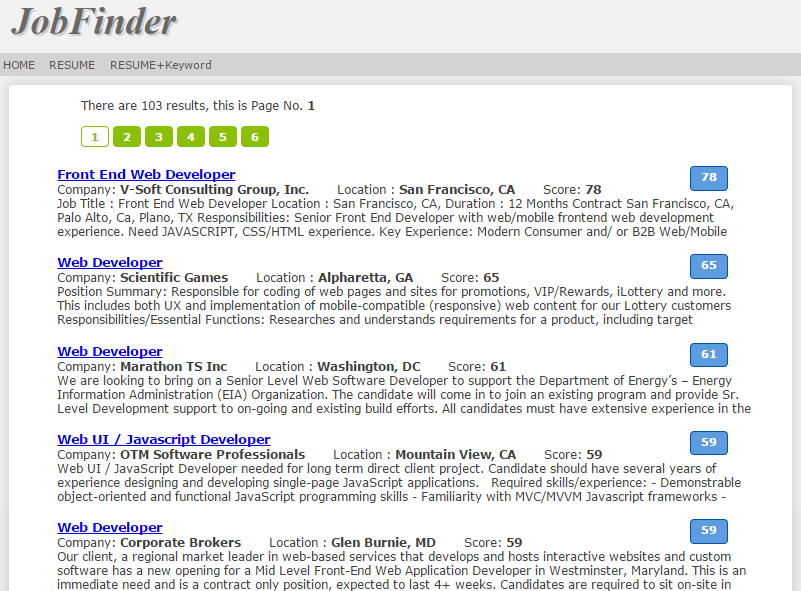
\includegraphics[scale=0.5]{images/match_resume.png}
  \caption{Jobs returned by the system}
  \label{fig:result}
\end{figure}

\subsection{System Architecture}

Figure~\ref{fig:Pipeline} shows the architecture of the whole system, which includes such modules:

\begin{enumerate}
    \item The Web Crawler can access and download all new IT job opening web pages from indeed.com everyday.
    \item The Job Parser can parse the job opening web pages, extract the information and create the job models.
    \item The Resume Parser is much like the Job Parser; it parses the r\'esum\'es and creates the r\'esum\'e models.
    \item All the job descriptions and job models are stored in the database.
    \item When a user searches  the jobs with their r\'esum\'e, the Ontology Matcher calculates the similarity values of jobs in the database and returns the jobs ranked by their similarity values.
\end{enumerate}

\begin{figure}[htbp]
  \centering
  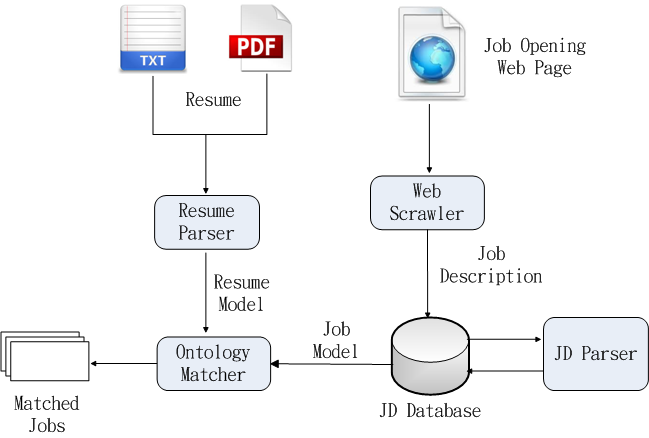
\includegraphics[scale=0.5]{images/arch.png}
  \caption{System Architecture}
  \label{fig:arch}
\end{figure}

\subsection{Text Processing Stages}

The Information Extraction framework in our system uses six stages in order to extract the information from job descriptions: HTML parsing, segmenting, preprocessing, tokenizing, labeling and pattern matching, which is show in Figure~\ref{fig:Pipeline}.

1) The \textbf{HTML Parsing} will parse the web pages that contain job descriptions, which are obtained from web crawler. The parser uses HTML tag template to extract attributes of the jobs, like job title, location, company name, content and so on. A job will be saved as a record with these attributes in the database. In the record, the content field contains the text part of the job description, which will be processed in later stages.

2) In the \textbf{segmenting stage}, the content field of the job description is be separated into paragraphs according HTML tags. Then paragraphs are separated into sentences by either HTML tags or punctuation, and after this step, all HTML tags will be removed.

3) Web pages of job description are created in different character sets, (e.g. UTF8 and ISO 8859-1), and almost always contain some unreadable characters. In the \textbf{prepossessing stage}, characters in the sentences are converted to ASCII characters, unreadable characters will be deleted, and some punctuation will be replaced by spaces (e.g. / and -).

4) In the \textbf{tokenizing stage}, the sentences will be tokenized into arrays of tokens by NLTK~\cite{bird2006nltk}.

5) In the \textbf{labeling stage}, the sentences will be given two layers of labels by a dictionary matching approach. The labels in the first layer are the semantic value of the text, and the labels in the second layer are the ontology hypernym of the labels in the first layers.

6) In the \textbf{pattern matching} stage, the FST library is used to matching the labels of the labeled sentences.  If a layered sentence match any pre-defined pattern, the information will be extracted and added to the job model. After every sentence of a job description has be processed, a job model will be created and saved in the database. More details about matching will follow in Section C.

\begin{figure}[htbp]
  \centering
  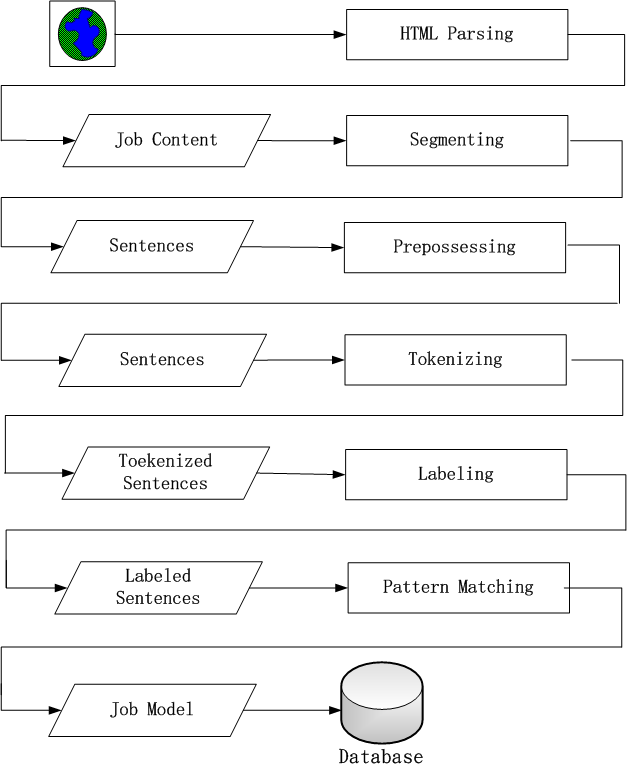
\includegraphics[scale=0.4]{images/pipeline2.png}
  \caption{Job Description Process Pipeline}
  \label{fig:Pipeline}
\end{figure}


\section{Information Extraction}
\label{sec1}

The IE framework will be introduced by example of processing the job descriptions. We use rule based method to extract the information from r\'esum\'es and job descriptions. To achieve this, we proposed  a Finite-State Transducer(FST) based pattern matching library. 

In natural language, a single concept often has multiple expressions to represent it. For example, the simple concept bachelor's degree,  can be expressed in many ways in job descriptions, e.g. B.S., BA/BS, 4-years-degree, and so on. Table \ref{tab:multispelling} shows the words that if followed with word ``degree'' have the semantic value of ``bachelor's degree''.

\begin{table}[ht]
\caption{All words mean bachelors} % title of Table
\centering % used for centering table
\begin{tabular}{  | p{15cm} |  }
 \hline
 "Baccalaureate","bachelors", "bachelor" ,"B.S.", "B.S","BS","BA","BA/BS", "BABS", "BSBA", "B.A." ,"4-year","4-year", "4 year", "four year","college","Undergraduate" , "University" \\
  \hline
\end{tabular}
\label{tab:multispelling} % is used to refer this table in the text\section{Pipeline of Information Extraction}
\end{table}

To add labels to a sentence, we use token pattern matching library which support a regular expression over tokens. If we use all the expressions of a semantic value to create a pattern, the pattern will be very large, and there are too many states in the FST. For example, if we use some words in Table~\ref{tab:multispelling} to create the pattern of semantic value ``bachelor's degree'', the pattern will like below:
$$ (~Baccalaureate~\mid~bachelors~\mid~bachelor~~\mid~B.S~\mid~BS~\mid~BA~)~~degree $$
If all words in Table~\ref{tab:multispelling} are added to the pattern, the FST will have too many edges, and the matching process will be very slow because of the problem of combinatorial explosion.

To resolve this problem, we proposed an approach to use the patterns to match the \textit{labels} of the tokens, not the the original text. In the system, we don't care what words the sentences really use, but want to extract the semantic value of the tokens which match the pattern. The details of the approach is described below.

At first, we created two dictionaries, which are used to label the tokens. In the first dictionary, the keys are the tokens, like words in Table~\ref{tab:multispelling}, and the values are the symbols for semantic values, like ``BS-LEVEL'' for ``bachelor's degree'', or ``MS-LEVEL'' for ``master's degree''. The values of the the second dictionary are the ontology hypernym of their keys, like keys ``BS-LEVEL'' and  ``MS-LEVEL'' both have value ``DE-LEVEL'', which means that bachelor's degree and master's degree are both one kind of degree level. We show the dictionaries for degree information in Table~\ref{tab:semanticlabeling}. There are also some words in the dictionaries that have the same first layer and second layer labels, which is shown in Table~\ref{tab:morelabels}.

\begin{table}[ht]
\caption{Semantic Labeling } % title of Table
\centering % used for centering table
\small
\begin{tabular}{  | l | l | l |   }
 \hline
 Original Text & Layer 1 & Layer 2  \\
 \hline
   bachelors  &  \multirow{4}{*} ~BS-LEVEL   & \multirow{10}{*} ~DE-LEVEL  \\
 \cline{1-1}
   bachelor   &     &    \\
 \cline{1-1}
   B.S.       &     &    \\
 \cline{1-1}
   Baccalaureate    &     &    \\
 \cline{1-2}
   Master     &  \multirow{3}{*} ~MS-LEVEL   &    \\
 \cline{1-1}
   MS         &     &    \\
 \cline{1-1}
   M.S.       &     &    \\
 \cline{1-2}
   PhD        &  \multirow{3}{*} ~PHD-LEVEL      &    \\
 \cline{1-1}
 Ph.D         &     &    \\
 \cline{1-1}
  Doctorate   &     &    \\
 \hline

\end{tabular}
\label{tab:semanticlabeling} % is used to refer this table in the text\section{Pipeline of Information Extraction}
\end{table}



\begin{table}[ht]
\caption{More Labels} % title of Table
\centering % used for centering table
\small
\begin{tabular}{  | l | l | l |    }
 \hline
 "Be", "be", "is", "are", "was", "were", "am"    &  ~BE          & ~BE     \\
 \hline
 "a", "A", "an", "An", "The", "the"              &  ~DE          & ~DE    \\
 \hline
 "MBA", "BSCS", "BSEE", "MSCS"                   & \multirow{2}{*}~MAJOR-DEGREE &  \multirow{2}{*}  ~MAJOR-DEGREE  \\

 "MSEE", "MSCE","MPH"     &   &  \\
 \hline
  "practical experience" , "work experience" & \multirow{2}{*}~EXPERIENCE  & \multirow{2}{*} ~EXPERIENCE  \\
  "professional experience", "experience��    &              &       \\
 \hline
 "preferred", "required", "desired"     &  ~PREFER-VBD  & ~PREFER-VBD    \\
 \hline
 "a plus", "mandatory", "desirable"     &  ~PREFER-JJ   & ~PREFER-JJ      \\
 \hline
 "similar", "related", "Relevant"    &  \multirow{2}{*}~DEGREE-JJ   & \multirow{2}{*}~DEGREE-JJ    \\
 "equivalent", "based"              &               &              \\
 \hline
\end{tabular}
\label{tab:morelabels} % is used to refer this table in the text\section{Pipeline of Information Extraction}
\end{table}


With the two dictionaries, we can label the tokens with two layers. Table~\ref{tab:labeldsent} shows how the sentence ``Bachelors  degree  in computer science or information systems.'' is labeled.

\begin{table}[ht]
\caption{Labeled sentence } % title of Table
\centering % used for centering table
\small
\begin{tabular}{  | c | c | c | c | c |c | c |c | c | c |  }
 \hline
 layer 2 & DE-LEVEL   & DEGREE & IN & MAJOR            & OR & MAJOR  &.  \\
 \hline
 layer 1 &  BS-LEVEL   & DEGREE & IN & MAJOR-CS         & OR & MAJOR-INFO & .      \\
 \hline
   words & bachelors   & degree & in & computer science & or & information systems & .     \\
  \hline
\end{tabular}
\label{tab:labeldsent} % is used to refer this table in the text\section{Pipeline of Information Extraction}
\end{table}

The pattern ``DE-LEVEL DEGREE  IN   MAJOR  OR  MAJOR ''  can match the sentence above, and the output of the matching process is ``BS-LEVEL'' for bachelor's degree, ``MAJOR-CS'' and ``MAJOR-INFO'' for two majors mentioned in sentence. In our system, most patterns match the labels in second layer. With this approach, the size of the FST for the pattern will be minimized, so speed of matching process can be improved.


\subsection{Patterns for Matching}
\label{subsec1}

As we explained in section B, we mentioned matching tokens in the second layer to patterns we defined. To match the labels in sentences to our patterns, we proposed a library that support matching pattern over tokens. The difference between this library and traditional regular expression is that the basic unit to be matched is token, not character. Some patterns used to match degree phrases are in Table~\ref{tab:patterns}. The patterns looks like regular expression, but they use tokens as the basic units.

\begin{table}[ht]
\small
\caption{Patterns to match degree sentences} % title of Table
\centering % used for centering table
\begin{tabular}{  | l  |  }
 \hline
 DE-LEVEL,  DE-LEVEL, OR  DE-LEVEL DEGREE   \\
 DE-LEVEL DEGREE ( IN  $\vert$  OF ) DT MAJOR   \\
 MAJOR-DEGREE  ,  MAJOR-DEGREE OR MAJOR \\
 DE-LEVEL (, DE-LEVEL)* (OR DE-LEVEL)? BE? PERFER-VBD   \\
 \hline
\end{tabular}
\label{tab:patterns} % is used to refer this table in the text\section{Pipeline of Information Extraction}
\end{table}


\subsection{Pattern Matching Library}
\label{subsec1}

Finite-State Transducers~\cite{roche1997finite} have been used as a tool to match patterns and extract information for more than 20 years. This approach has been demonstrated to be very effective in extracting information from text like CIRCUS~\cite{lehnert1991university} and FASTUS~\cite{hobbs199713}.  In the widely used NLP toolkit GATE~\cite{cunningham2002framework}, the semantic tagger JAPE (Java Annotations Pattern Engine) could describe patterns that are used to match and annotate tokens. JAPE adopts a version of CPSL (Common Pattern  Specification Language)~\cite{appelt1998common}, which provides FST over annotations. Chang et al. presented cascaded regular expressions over tokens~\cite{chang2014tokensregex}, which proposed a cascaded pattern matching tool over token sequences.

After studying these tools, we found most of them to be powerful and complex, but not very flexible. One reason is that developers need to learn some Domain specific Languages (DSLs) like CPSL. The other reason is the extra effort and time required to integrate the pattern matching tool into the system. So here we proposed a more flexible and lightweight FST framework, which can do regular expression matching over labeled tokens. We give the definition of Finite-State Transducer here. A Finite-State Transducer is a 6-tuple $(\Sigma_1, \Sigma_2, Q, i, F, E)$ where:
\begin{itemize}
  \item $\Sigma_1$ is a finite alphabet, called the input alphabet.
  \item $\Sigma_2$ is a finite alphabet, called the output alphabet.
  \item Q is a finite set of states.
  \item $i \in Q$ is the initial state.
  \item $F \subset Q$ is the set of final states.
  \item $E \subset  Q  \times \Sigma_1^* \times \Sigma_2^* \times Q$ is the set of edges.
\end{itemize}

Regular expressions can be converted to automata \cite{aho1992foundations}, and FST is also an automata. To convert a regular expression over token to a FST we need two steps: The first is parsing the expression to a tree of matchers, the second is transfer the tree of matchers to the FST. We will introduce these two steps in next.

In our library, a ``matcher'' could be a token to be matched, or a composition of other matchers. Our library supports syntax used in traditional regular expressions over strings. We list the syntax that the library supports in Table~\ref{tab:matchers}. The first column is the names of the matchers, the second column is the explanation of the function of the matchers, and third column is the their counterpart syntaxes of traditional regular expression. The RegexMatcher in our library is constructed with a regular expression, and the matcher matches any string that matches the regular expression in the matcher. We give examples of the syntax of these matchers in Table \ref{tab:matchers_example}.

\begin{table}[ht]
\caption{Matchers of our Library } % title of Table
\centering % used for centering table
\begin{tabular}{  | l | l | l |  }
 \hline
 Matcher Name      &  Function                                 & Counter Part of regex    \\
 \hline
 UnitMatcher       &  token is matches the it                  & character  in regex       \\
 \hline
 SequenceMatcher   &  A list of Matcher                        & sequence of characters       \\
  \hline
 QuestionMatcher   &  One or more of the preceding token       & ?       \\
  \hline
 StarMatcher       &  Zero or more of the preceding token      & *       \\
  \hline
 PlusMatcher       &  Zero or one of the preceding token       & +       \\
  \hline
 DotMatcher        &  Any token                                & .      \\
  \hline
 RegexMatcher      &  Any token matches the regular expression               &  N/A      \\
  \hline
\end{tabular}
\label{tab:matchers} % is used to refer this table in the text\section{Pipeline of Information Extraction}
\end{table}



\begin{table}[ht]
\caption{Matchers' Examples } % title of Table
\centering % used for centering table
\begin{tabular}{  | l |  l |  }
 \hline
 Matcher Name          & Example    \\
 \hline
 UnitMatcher         & DEGREE       \\
 \hline
 SequenceMatcher     & DE-LEVEL DEGREE       \\
  \hline
 QuestionMatcher     & DE-LEVEL (OR DE-LEVEL)?  DEGREE       \\
  \hline
 StarMatcher         & DE-LEVEL (, DE-LEVEL)*  DEGREE       \\
  \hline
 PlusMatcher         & DEGREE IN MAJOR +      \\
  \hline
 DotMatcher          & HAS . DEGREE      \\
  \hline
 RegexMatcher        & r``d-d'' years  \\
  \hline

\end{tabular}
\label{tab:matchers_example} % is used to refer this table in the text\section{Pipeline of Information Extraction}
\end{table}

The framework supports three styles of creating patterns: regular expression style, operator style and object style. The second and third styles are flexible because developers can create their own matcher class to extend the feature of the library. We use examples to show how the three styles work. The most common style is defining pattern expression in a string, which is much like traditional regular expression.

\begin{framed}
\small
\noindent
The pattern is:  DE-LEVEL DEGREE ( IN  $\vert$  OF ) DT? MAJOR \\
The code is: \\
seqMatcher =parser.parse("DE-LEVEL DEGREE ( IN  $\vert$  OF ) DT? MAJOR")

\end{framed}

The second style is using algebraic operators to connect matchers, which can help developer reuse previous patterns when the new patterns include old ones. It is shown in follows:
\begin{framed}
\small
\noindent
The pattern is:  "DE-LEVEL DEGREE (IN $\vert$ OF) MAJOR" \\
The code is: \\
seqMatcher =  UnitMatcher("DE-LEVEL") +  UnitMatcher("DEGREE") + \\
\hspace{3cm} ( UnitMatcher("IN") $\vert$ UnitMatcher("OF" ) ) + UnitMatcher("MAJOR")

\end{framed}

We also could create a complex matcher in object-oriented programming style.

\begin{framed}
\small
\noindent
The pattern is:  "DE-LEVEL DEGREE (IN $\vert$ OF) MAJOR" \\
The code is: \\
matcher1 = UnitMatcher("DE-LEVEL") \\
matcher2 = UnitMatcher("DEGREE")  \\
matcher3 = UnitMatcher("IN")   \\
matcher4 = UnitMatcher("OF")   \\
matcher5 = UnitMatcher("MAJOR")  \\
matcher6 = AlternateMatcher([matcher3,matcher4])   \\
seqMatcher = SeqMatcher([matcher1, matcher2, matcher6, matcher5])

\end{framed}

The flexibility of the tool also comes from the fact that developers can determine which layer of the array should be matched, the original text, or labels in the first layer or labels in the second layer. Developers can assign a lambda expression to the matcher's catching function, which defines how to get the matching input strings from the sentences, as well as an out function, which defines what should be outputed. For example,  the labeled sentence is a sequence of arrays, each array includes the original text token and its labels in the other two layers, which is shown in table~\ref{tab:labeldsent}. To match the labeled sentence, we set the lambda expression for catching function to ``lambda x:x[2]'', and the out function to ``lambda x:x[1]'', which make the matcher match the label in second layer, and output the the value of semantic value in the first layer.

\subsection{Evaluation}

To evaluate the performance of the information extraction module, we extract sentence types through the use of sentence filters. To explain the process of our experiment, we use the sentences whose content pertains to the applicant's college degree information.

In the experiment, we selected 100 sentences from existing job descriptions, and the content of these sentences were requirements of candidate degree and major. We labeled the values for "degree" and "major" manually. We use some content patterns that we can identify from these sentences to match and extract the degree information. When we used 6 patterns, the accuracy of "degree" became 94\%. We also compared our pattern matching method to the conditional random fields (CRFs) model~\cite{lafferty2001conditional}, which is a state of art machine learning model for sequence labeling. We used 200 labelled sentences to train the CRF model, and the features of the CRF model are words in the sentences and part of speech tags of the words. The accuracies of information extraction of the three fields with our two methods, pattern matching, and the application of the CRF model are shown in Table \ref{tab:ieaccura}.


\begin{table}[ht]
\caption{Information Extraction} % title of Table
\centering % used for centering table
\begin{tabular}{   | c | c | c | c |   }
 \hline
          Field   & Pattern Num & Accuracy of Pattern Matching  & Accuracy of CRF   \\
 \hline
          Degree  & 6           & 0.94       &  0.85  \\
 \hline
          Major   & 10          & 0.85       &  0.72  \\
 \hline

\end{tabular}
\label{tab:ieaccura} % is used to refer this table in the text
\\Our pattern matching approach can get higher accuracy.
\end{table}


\section{Model Similarity}
\label{sec1}

The similarity value between a  job model and a r\'esum\'e model is the summation of weighted similarity values of different fields. The equation is given below:
$$ sim(r, j) = \sum_{i=1}^{n} simfun_i(r_i,j_i) \times w_i $$
The value of $sim(r, j)$ is the summation of similarity values of different fields times their corresponding weights. $simfun_i(r_i,j_i)$ is the similarity function of the $ith$ field of the model. In our system, the r\'esum\'e model and job model both have four fields: job title, major, academic degree and skills. The similarity value between a r\'esum\'e model and job model is the sum of the productions of similarity values of all the fields pairs and their weights. We will introduce how to calculate the similarity value for each field in this section.
 
\subsection{Similarity of Major and Academic Degree}

In the simplest case, if the majors in the r\'esum\'e model and job model are the same, the similarity value is 1. If they are different, we can check whether the major in the r\'esum\'e model is in the list of related majors for the major in the job model. If it is, the similarity value is 0.5; otherwise the similarity value is 0. The equation is shown below:

$$ MajorSim(r,j ) = \begin{Bmatrix}
1, & r_{major} = j_{major} \\
0.5, & r_{major} \in related( j_{major} ) \\
0, & otherwise
\end{Bmatrix} $$

There are five kinds of academic degrees in the system:  high school, associate, bachelor, master, and Ph.D., which are mapped to the integer values form 1 to 5. If the degree value in the r\'esum\'e model is less than that in the job model, which means that the job seeker's education background cannot satisfy the requirement of the job, the similarity value in this case is 0. If the degree value in the r\'esum\'e model is equal to the job model and no more than 2 above, the similarity value is 1. In some cases, the degree value in the r\'esum\'e model is greater than that of the job model, and the difference is greater than 2, which means that the job seeker's degree is much higher than the requirement of the job. The situation is also a kind of relative matching, so the similarity value here is 0.5. The equation is shown below:

$$ DegreeSim(r,j ) = \begin{Bmatrix}
0,   & r_{degree} < j_{degree} \\
1,   & 0 < r_{degree} - j_{degree} \leqslant 2  \\
0.5, & r_{degree} - j_{degree} > 2
\end{Bmatrix} $$

\subsection{Similarity of Job Title}
Another field of needs similarity calculation is the job titles in the models. A job title can be parsed into some sub fields: job role, level, platform, programming language.  The value of job roles includes: developer, manager, administrator and so on. There are levels values in such roles: such as junior, senior and architect. The platforms: web, mobile and cloud are used by the very roles.  The similarity value between two titles is the sum of all the similarity values of these fields. The similarity value of each sub filed ranges from 0 to 1, and we also normalized the similarity summation value to 1 by dividing the number of sub fields. If the job seeker has some working experience, there may be some job titles in their r\'esum\'e.  When calculating the similarity value between a r\'esum\'e model and a job model, the system calculates the similarity values of the title of job model to all the titles in the r\'esum\'e model and returns the maximum one.

\subsection{Similarity of Skills}

The job model usually has requirements of some skills, and the r\'esum\'e model lists the skills the job seeker has as well. The similarity value of skills field is the summation of all the similarity values of skills in the job model. For every skill in the job model, the similarity value is the maximum value it can get from the skills in the r\'esum\'e model. The equation is shown below:

$$ SkillSim(sj_i,SR ) = \begin{Bmatrix}
1, & sj_i \in SR  \\
max( sim (sj_i, rj_k )), & sj_i \notin SR \\
\end{Bmatrix} $$

In the equation, $sj_i$ is the $i$th skill in the job model, and $SR$ is the skill set of the r\'esum\'e model. If there is the skill $sj_i$ in the skill set $SR$, the similarity value for $sj_i$ is 1, otherwise the system chooses the maximum similarity value from all the similarity values between skill $sj_i$ and the skills in the the r\'esum\'e model.
 
\section{Ontology Construction and Similarity}
\label{sec1}
 
After getting job models by the information extraction module, users can search for jobs in the system. In the system, ontology is used as a knowledge base to store knowledge and rules, which could help compare the similarity between different concepts.

\subsection{Ontology Construction}

Before calculating the similarity between concepts, we need to construct the ontology first. Semantic web has been a popular research topic in previous years, and at the same time thousands of domain ontologies have been created~\cite{ding2004swoogle}. A paradigmatic example is WordNet~\cite{fellbaum1998wordnet}, which is a general purpose thesaurus, and contains more than 100,000 general English concepts. ACM has created a poly-hierarchical ontology that can be utilized in semantic web applications~\cite{acm2012class}, but it is mostly used in academic areas. DBpedia~\cite{bizer2009dbpedia} provides structured information from Wikipedia and make this information available on the Web, but its coverage is huge, and most of them is not related to job finding. Currently, there is no domain specific technology ontology built for recruiting purpose.

The domain specific technology ontology for recruiting should include a lot of technical terms, like programming language, programming library, commercial products and so on. Furthermore, there are new techniques invented everyday, so new IT terms will appear continuously. Ding et al.~\cite{ding2002ontology} gave a survey of current ontology generation approaches such as manual, semi-automatic, and automatic. Some aspects of the approaches were discussed in the paper, like the source data, concept extraction methods, ontology representation, and construction tools. Inspired by this paper, we propose a semi-automatic approach to construct the IT skill ontology, which use a pattern matching approach to collect possible technical terms, and use DBpedia to verify the them.

From the observation, we found that sentences with skill requirements in job descriptions always list several skills in the sentence, which is shown in Table ~\ref{tab:skillrequirement}. Based on this character, we propose a bootstrap approach to collect IT terms in job descriptions.  First, we manually collect about fifty terms from job descriptions, and add them to the term list. Then we use our pattern match library to find the sentences that matching the pattern in Table \ref{tab:patterns} from a set of job descriptions. An example of a sentence which matches the pattern is shown in Table \ref{tab:termspattern}. We extract the tokens which match the star symbol from the sentences; these tokens have high probability to be technical terms. Then we could check the tokens in Dbpedia to see whether they are under the categories like software, programming language or any other technical related ones. If they are, we could classify them as terms, and add them to the terms list. After scanning all the sentences in the job description set, the term list will be larger, and we can use the larger term list to start a new iteration of scaning. This process stops when the number of found new terms is below a threshold. The process is shown Figure~\ref{fig:gen_onto}.

\begin{table}[ht]
\caption{Example Sentences in Job Descriptions} % title of Table
\centering % used for centering table
\begin{tabular}{ | p{15cm}  | }
 \hline
    1. A high-level language such as Java, Groovy, Ruby or Python; we use Java and Groovy extensively \newline
    2. HTML5/CSS3/JavaScript, web standards, jQuery or frameworks like AngularJS would be great \newline
    3. HTML CSS and Javascript a must  \newline
    4. Experience with AJAX, XML, XSL, XSLT, CSS, JavaScript, JQuery, HTML and Web Services   \\
 \hline
\end{tabular}
\label{tab:skillrequirement} % is used to refer this table in the text
\end{table}



\begin{table}[ht]
\caption{Patterns to extract terms} % title of Table
\centering % used for centering table
\begin{tabular}{   | p{8cm} |  }
 \hline
     term   , * , *,  term  \\  \hline
     term  , * , *, and  term   \\
 \hline
\end{tabular}
\label{tab:patterns} % is used to refer this table in the text
\end{table}

\begin{table}[ht]
\caption{An example sentence matches the pattern} % title of Table
\centering % used for centering table
\begin{tabular}{   | c | c | c | c |c | c |c | c |c | c |c | c |c | c |  }
 \hline
     Experience & with & TERM & , & *   & , & *   &, & TERM &, & and & *  \\
 \hline
     Experience & with & AJAX & , & XML & , & XSL &, & XSLT &, & and & CSS  \\
 \hline
\end{tabular}
\label{tab:termspattern} % is used to refer this table in the text
\end{table}

For example, we extract the token  ''XSL'', which currently is not in the terms list. We check the word on DBpedia by accessing the URL:http://dbpedia.org/page/XSL. If we can get the XML formatted description of XSL, and any element in ``dcterms:subject'' section has the value which is a technical category,  like ``Programming languages'', ``Markup languages'' and so on, we can indicate that the word is a technical term, and add it to the term list.

\begin{figure}[htbp]
  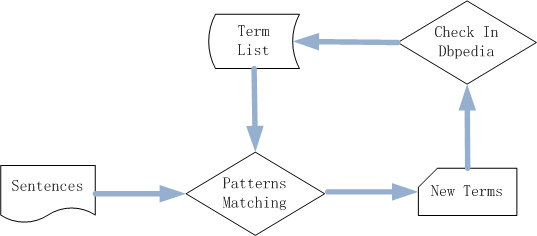
\includegraphics[scale=0.6]{images/genonto.png}
  \caption{Procedure of Finding Technical Terms}
  \label{fig:gen_onto}
\end{figure}

But not all the extracted terms can be verified in DBpedia, because some terms have multiple meanings in English, and the URLs of their DBpedia pages are unpredictable. For example, the word ``Python'' could be an animal name or a programming language.  The meaning of the programming language  has the DBpedia URL http://dbpedia.org/page/Python\_(programming\_language), which is difficult to predict. In this case, we have to check the term manually.  After getting all terms, we use Protege~\cite{noy2001creating}, an open source ontology editor, to edit the domain specific ontology, and saved it in RDF format. Part of the technical ontology is shown in Figure~\ref{fig:ontology_pro}.


\begin{figure}[htbp]
  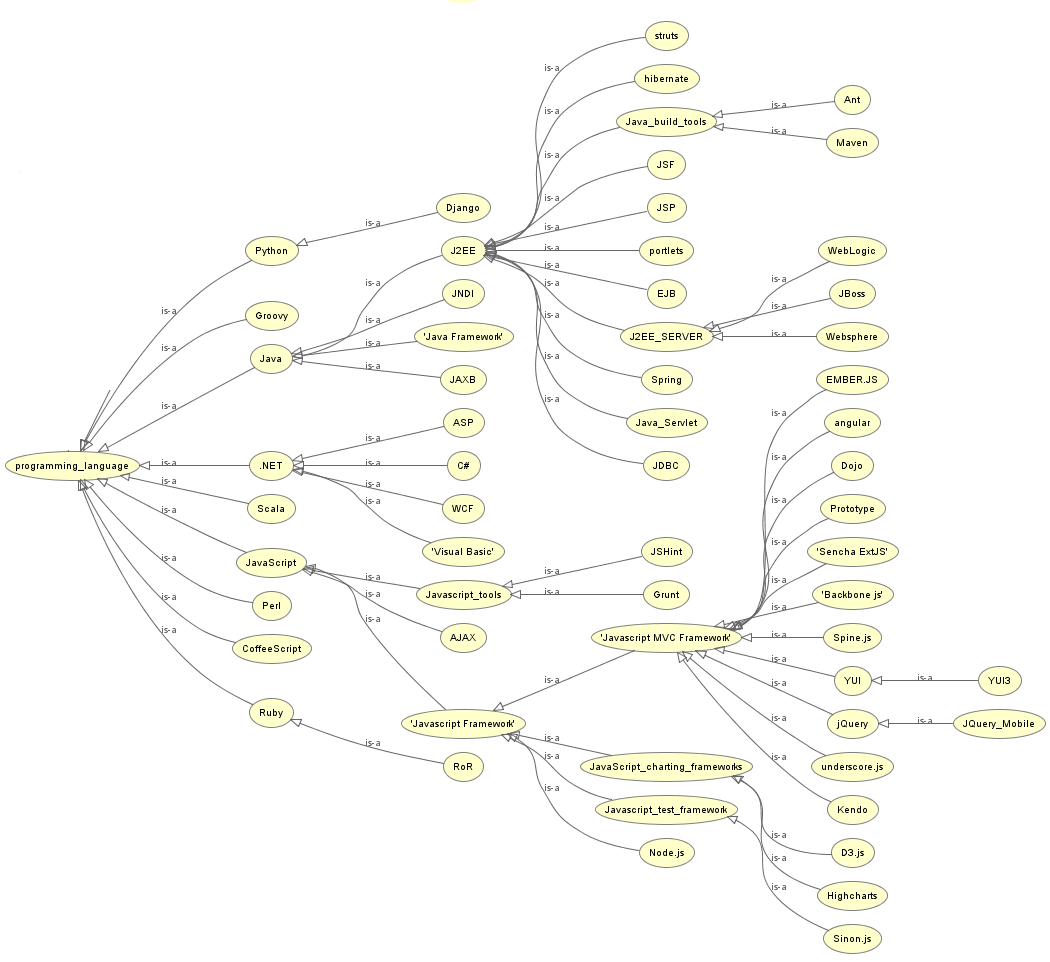
\includegraphics[scale=0.6]{images/ontology_pro.png}
  \caption{Part of Ontology}
  \label{fig:ontology_pro}
\end{figure}

\subsection{Ontology-based semantic similarity}

S{\'a}nchez et al. \cite{sanchez2012ontology} summarized ontology-based similarity assessment into three kinds and gave both advantages and disadvantages of each approach. The three kinds of categories are: Edge-counting approaches, Feature-based measures, and Measures based on Information Content.

In path-based approaches, the ontology is viewed as a directed graph, in which the nodes are the concepts, and the edges are taxonomic relation (e.g. is-a). Rada, et al.~\cite{rada1989development} measure the similarity by the distance of two nodes in the graph. Wu and Palmer~\cite{wu1994verbs} realized that the depth in the taxonomy will impact the similarity measure of two nodes, because the deeper of the nodes are in the tree, the semantic distance is smaller. Based on the same idea, Leacock and Chodorow~\cite{leacock1998combining} also proposed a similarity measure that combined distance   between terms and the depth of the taxonomy. There are some limitations of path-based approaches. First, it only considers the shortest path between concept pairs. When they meet a complex situation like multiple taxonomical inheritance, the accuracy of them will be low. Another problem of the path-based approaches is that they assume that all links in the taxonomy have uniform distance.

Feature based approaches assess the similarity between concepts as a function of their properties. They consider the degree of overlapping between sets of ontological features, like Tversky's model~\cite{tverskyfeatures}, which subtracts the non-common features from common features of two concepts. 
Rodr{\'\i}guez and Egenhofer~\cite{rodriguez2003determining} computed similarity by summing the weighted sum of similarities between synsets, features, and neighbour concepts. The feature-based methods consider more semantic knowledge than path-based methods. But only big ontologies/thesauri like Wordnet~\cite{miller1995wordnet} have this kind of information. Ding et al.~\cite{ding2004swoogle} revealed that domain ontologies very occasionally model any semantic feature apart from taxonomical relationship.


Other approaches want to overcome the limitations of edge-counting approaches are Content-based measures. Resnik~\cite{resnik1995using} proposed a similarity measure, which depends on the amount of shared information between two terms. Lin \cite{lin1998information} and Jiang and Conrath \cite{jiang1997semantic} extended Resnik's work. They also considered the IC of each of the evaluated terms, and they proposed that the similarity between two terms should be measured as the ratio between the amount of information needed to state their commonality and the information needed to fully describe them. The are also two disadvantages of the content-based measures. First, the approaches cannot compute the concepts of leave nodes, because they don't have subsumers. Second, if the concepts do not have enough common subsumers, their similarities are hard to be calculated.


\subsection{Statistical-based Ontology Similarity Measure }
In this paper, we proposed a new statistical-based ontology similarity measure. In most job descriptions, they list many skills the positions required. From observation, we found that related skills always exist in the job description simultaneously, and the positions of them are always close, e.g. HTML and CSS are always required together, and appear in the same sentence. We can see from the Table~\ref{tab:skillrequirement}, the closely related concepts are always have short distance. Based on such observation, we give a new statistical-based ontology similarity measure. If two concepts $a$ and $b$ have the same direct hypernym or one  is the hypernym of the other, the similarity between them is given:
$$ S(a,b) = \frac{  N_{a \cap b} / N_{a \cup b} }{avg(\log_2( mindis(d_i,a,b) + 1 ))} $$

The numerator is the ratio of the number of documents in which the two terms exist together $(N_{a \cap b})$ and the number of documents have a least one of them $(N_{a \cup b})$. The denominator is the average $\log$ value of minimum distance $mindis(doc,a,b)$ of the two terms in documents that have them both.

We set the restriction on the position of the two concepts in the ontology, because the position of the concepts in the ontology are based on their technical similarity to others. Similar techniques will be assigned into the same category, so they should share the same hypernym, and one could be an alternative to the other. For example, we put EJB and Hibernate in the same category, because they are both J2EE persistence layer technologies, and both have the O/R mapping concept. If the applicant is familiar one of them, they can master the other very quickly. Another example is Grail and Django, they are both web frameworks and share same web design philosophies, but one of them is designed for Java web application and the other is created for Python web application. If a developer has some some experience with one of them, he/she still need to spend a lot of time to learn the other to overcome the gap between programming languages. 

The matrix in Table~\ref{tab:dismatrix1} show the similarity values among of some skills, which is gotten from 500 job descriptions. For example the skill HTML, the most relevant skills in order are CSS, Javascript, and jQuery,  which is the same from the perspective of experienced developers. The other example is Java, the most relevant skill in the matrix is JSP, which is also agree with the general technical knowledge.


\begin{table}

\caption{Similarities of Skills List 1}
\begin{tabular}{ c | c c c c c c   }
 \hline
  Term       &  Java  &  JDBC  & Spring & Hibernate & MySql  & Oracle   \\  \hline
  Java   &   1    & 0.0523 & 0.091  &   0.0458  & 0.0339 & 0.0608    \\  \hline
    JDBC   & 0.0523 &   1    & 0.0525 &   0.0799  & 0.006  & 0.0616   \\  \hline
   Spring  & 0.091  & 0.0525 &   1    &   0.2008  & 0.0194 & 0.0878   \\  \hline
 Hibernate & 0.0458 & 0.0799 & 0.2008 &     1     & 0.0073 & 0.115    \\  \hline
   MySql   & 0.0339 & 0.006  & 0.0194 &   0.0073  &   1    & 0.049    \\  \hline
   Oracle  & 0.0608 & 0.0616 & 0.0878 &   0.115   & 0.049  &   1      \\  \hline
 \hline
\end{tabular}
\label{tab:dismatrix1}
\end{table}


\begin{table}

\caption{Similarities of Skills List 2}
\begin{tabular}{ c | c c c c c c c c }
 \hline
  Term       & Javascript & jQuery &  HTML  &  CSS   &  Java  & Python &  Ruby  &  JSP    \\  \hline
  Javascript &     1      & 0.1981 & 0.2087 & 0.2439 & 0.0665 & 0.0189 & 0.023  & 0.0253   \\
    jQuery   &   0.1981   &   1    & 0.0979 & 0.1328 & 0.0439 & 0.0142 & 0.0266 & 0.0232    \\
     HTML    &   0.2087   & 0.0979 &   1    & 0.3569 & 0.0473 & 0.0175 & 0.023  & 0.0103   \\
     CSS     &   0.2439   & 0.1328 & 0.3569 &   1    & 0.0537 & 0.0153 & 0.0181 & 0.015    \\
     Java    &   0.0665   & 0.0439 & 0.0473 & 0.0537 &   1    & 0.0498 & 0.0287 & 0.075    \\
    Python   &   0.0189   & 0.0142 & 0.0175 & 0.0153 & 0.0498 &   1    & 0.1333 & 0.0025   \\
     Ruby    &   0.023    & 0.0266 & 0.023  & 0.0181 & 0.0287 & 0.1333 &   1    & 0.012    \\
     JSP     &   0.0253   & 0.0232 & 0.0103 & 0.015  & 0.075  & 0.0025 & 0.012  &   1      \\
 \hline
\end{tabular}
\label{tab:dismatrix2}
\end{table}


\subsection{Experiments of Ontology Similarity}

We selected some common skills from 500 job descriptions; table~\ref{tab:dismatrix3} shows similarity values between these skills. Higher values correspond to greater similarities, so the similarity between one skill and itself is 1. We selected one concept and ranked the other concepts by their similarity values to this concept. Human judges helped rank these concepts by assigning them "relevance scores" so that we can use NDCG to evaluate the effectiveness of our approach.

We use the $ Normalized~Discounted~Cumulative~Gain ( NDCG )$ ~\cite{manning2008introduction} to evaluate the statistical-based similarity. NDCG is an important measure to evaluate the ranked retrieval results, which is the ratio of  Discounted Cumulative Gain ( DCG ) to Ideal Discounted Cumulative Gain ( IDCG ).
 $$ NDCG = \frac {DCG}{IDCG} $$

DCG is the measure of how documents are ranked according to their relevance scores, and IDCG is the DCG value that the documents are strictly sorted by their relevance values.
$$DCG =  \sum_{i=1}^{p} \frac {2^{rel_i} - 1}{\log_2(i+1)} $$

Table~\ref{tab:simcompare1} shows how we evaluate the similarity between the concept ``Javascript'' and other concepts. The first column is a skill name, the second column is its similarity value to ``Javascript'', the third column is its position ranked by the similarity value, and the fourth column is its relevance value given by the judges. The NDCG value for concept Javascript is 0.94, and in Table~\ref{tab:simcompare2},  NDCG value for concept HTML is 0.97. They both hare relative high value.

\begin{table}
\centering
\caption{ Javascript Similarity Evaluation : NDCG = 0.94 }
\begin{tabular}{ | c | c | c  | c |  }
 \hline
    Term     &  Similarity Value  &  Position   & Relevance     \\  \hline
    jQuery   &  0.1981            &      4      &   8        \\
     HTML    &  0.2087            &      3      &   4         \\
     CSS     &  0.2439            &      2      &   3   \\
     Java    &  0.0665            &      5      &   1   \\
    Python   &  0.0189            &      8      &   1   \\
     Ruby    &  0.023             &      7      &   1    \\
     JSP     &  0.0253            &      6      &   2    \\
 \hline
\end{tabular}
\label{tab:simcompare1}
\end{table}


\begin{table}
\centering
\caption{ HTML Similarity Evaluation : NDCG = 0.97 }
\begin{tabular}{ | c | c | c  | c |  }
 \hline
    Term      &  Similarity Value  &  Position   & Relevance     \\  \hline
  Javascript   &  0.2087           &      2      &   3        \\
     jQuery    &  0.0979           &      3      &   3         \\
     CSS     &  0.3569             &      1      &   5   \\
     Java    &  0.0473             &      4      &   1   \\
    Python   &  0.0175             &      6      &   1   \\
     Ruby    &  0.023              &      5      &   1    \\
     JSP     &  0.0103             &      7      &   3    \\
 \hline
\end{tabular}
\label{tab:simcompare2}
\end{table}


\section{Evaluation of the System}
\label{sec1}

\subsection{Comparing with other models}

In a traditional information retrieval systems, Precision@K and NDCG are widely used measures. 
Precision@K is the proportion of relevant documents in the first K positions and is given below:
$$ P@k = \frac{1}{k} \sum^m_{i=1} l_i 1 \left(  r(i) \leq k  \right )  $$
Where 1 is the indicator function: $1(A) = 1$ if A is true, 0 otherwise.

To evaluate a job finding, we compare the results of the system with three classical information retrieval models: Kullback-Leibler divergence~\cite{zhai2008statistical},  TF-IDF~\cite{manning2008introduction} and Okapi BM25~\cite{robertson1995okapi}. We give the definition of these measures below.

Kullback-Leibler divergence is a non-symmetric measure of the difference between two probability distributions $P$ and $Q$. The score of a document $D$ with respect to query $Q$ is given by:
\begin{equation}
    \begin{array}{rcl}
        s(D,Q) & = & -D( \theta_Q \parallel  \theta_D )\\
               & = &- \sum_{ \omega \in V } p (\omega \mid \theta_Q) \log \frac{ p (\omega \mid \theta_Q )}{p(\omega \mid \theta_D)} \\               

    \end{array}
\end{equation}

In the equation $\theta_Q$ is the language model for a query, and  $\theta_D$ is the language model for a document.

TF-IDF is a Vector Space Model, which calculates the similarity between the vectors of the query $q$ and the document $d$. In the equation, $tf$ is the term frequency, and $idf$ is the inverse document frequency. The TF-IDF weighting scheme assigned to term $t$ a weight in document $d$ given by:
$$ tf\text{-}idf_{t,d} = tf_{t,d} \times idf_{t} $$
The similarity between the query $q$ and the document $d$ given by:
$$ score(q,d) =  \sum_{t \in q }  tf\text{-}idf_{t,d} $$

Okapi BM25 is a bag-of-words retrieval model that ranks a set of documents based on the query terms appearing in each document. Given a query $q$, the BM25 score of a document $d$ is:

$$ score(q,d) = \sum_{ t \in q  }  idf_t \frac {tf_{t,d} \cdot(k_1 +1) }  {tf_{t,d} +k_1 \cdot ( 1-b + b\cdot \frac { \left | D \right |}{avgdl})}  $$

In the formula, $idf_t$ is IDF value of term $t$, $tf$ is the term frequency; $ |D|$ is the length of the document $D$; $avgdl$ is the average length of all the documents, and $k_1$ and $b$ are the free parameters.

In the evaluation phase, we created a data set of 100 job descriptions that includes several kinds of jobs such as web developers, server back-end developers, mobile developers and so on. We used 5 candidate r\'esum\'es and retrieved the top 20 jobs.  The relevance value of the job descriptions to each r\'esum\'e were set manually by ten human judge. We created a query $q$ from the r\'esum\'e, treated the text of the job descriptions as documents $d$, and applied standard ad-hoc retrieval techniques to rank the jobs. We intended to return jobs that better matched the candidates' r\'esum\'es at the top. The result of Precision@k is in table~\ref{tab:job_precision}.


\begin{table}[ht]
\caption{Precision of Job Ranking } % title of Table
\centering % used for centering table
\begin{tabular}{    | c | c | c | c | c |  }
 \hline
       k     & Okapi BM25 & KL    & TF-IDF   & Our system  \\
 \hline
       5     & 0.66       & 0.27  & 0.72     & 0.82   \\
 \hline
       10    & 0.46       & 0.27  & 0.50     & 0.76   \\
 \hline
       20    & 0.33       & 0.21  & 0.35     & 0.77   \\
 \hline

\end{tabular}
\label{tab:job_precision} % is used to refer this table in the text
\\Our system get the highest precision.
\end{table}

The other measure we used is NDCG, which is explained in last section. Table~\ref{tab:job_ndcg} shows the NDCG value get from different information retrieval models. The result shows that Ontology Similarity  performs the best.

\begin{table}[ht]
\caption{NDCG of Job Ranking } % title of Table
\centering % used for centering table
\begin{tabular}{    | c | c | c | c | c |  }
 \hline
       k    & Okapi BM25 & KL    & TF-IDF & Our system  \\
 \hline
       5    & 0.15       & 0.34  & 0.45     & 0.78   \\
 \hline
       10   & 0.18       & 0.44  & 0.47     & 0.72   \\
 \hline
       20   & 0.19       & 0.35  & 0.45     & 0.66   \\
 \hline

\end{tabular}
\label{tab:job_ndcg} % is used to refer this table in the text
\\Our sytem get the highest NDCG value.
\end{table}

\subsection{Comparing with the Keyword Searching}
We also made experiments to compare the quality of search results quality between our system and the keyword searching approach. In one experiment, we first selected a r\'esum\'e, and picked a related keyword e.g. ``Java''  to search jobs in Indeed.com. We used this process to simulate how a job seeker searches jobs on Indeed.com. The top 100 jobs returned by Indeed.com were saved in our system, then we used the r\'esum\'e to match the 100 jobs. We compared the quality of the approaches by calculating the measures Precision@K  and  DCG. We use DCG not NDCG because we compare the two approaches on the same data set, and the IDCG is the same. Five judges gave the relevance values to the r\'esum\'es and jobs, and we used average values. Table~\ref{tab:comparison_java} shows comparison between the two approaches by using keyword ``Java'' and the r\'esum\'e of a Java developer. The comparison for  keyword ``Python'' and the r\'esum\'e of a Python developer is shown in Table~\ref{tab:comparison_python}, and the average comparison for five keywords and five r\'esum\'e is shown in Table~\ref{tab:comparison_avg}. We can see from the result that our system can get much better results than keyword searching approach.

\begin{table}[ht]
\caption{Comparison of the Two Approaches - Java Developer  } % title of Table
\centering % used for centering table
\begin{tabular}{    | c | c | c | c | c |  }
 \hline
  \multirow{2}{*}k    & \multicolumn{2}{c|}{Precision@K }    & \multicolumn{2}{c|}{DCG } \\
 \cline{2-5}
            & Indeed  & Our System  & Indeed     & Our System   \\
 \hline
       5    & 0.7     & 1               & 10.86       & 27.785   \\
 \hline
       10   & 0.65    & 0.95            & 24.85       & 47.06   \\
 \hline
       20   & 0.7     & 0.825           & 51.97       & 73.33   \\
 \hline

\end{tabular}
\label{tab:comparison_java} % is used to refer this table in the text
\\Our system can get better result.
\end{table}



\begin{table}[ht]
\caption{Comparison of the Two Approaches - Python Developer  } % title of Table
\centering % used for centering table
\begin{tabular}{    | c | c | c | c | c |  }
 \hline
  \multirow{2}{*}k    & \multicolumn{2}{c|}{Precision@K }    & \multicolumn{2}{c|}{DCG } \\
 \cline{2-5}
            & Indeed  & Our System  & Indeed     & Our System   \\
 \hline
       5    & 0.4    & 0.6               & 11.27       & 11.98   \\
 \hline
       10   & 0.3    & 0.6               & 13.43       & 15.79   \\
 \hline
       20   & 0.2    & 0.4               & 16.44       & 20.21   \\
 \hline

\end{tabular}
\label{tab:comparison_python} % is used to refer this table in the text
\\Our system can get better result.
\end{table}

\begin{table}[ht]
\caption{Comparison of the Two Approaches - Average  } % title of Table
\centering % used for centering table
\begin{tabular}{    | c | c | c | c | c |  }
 \hline
  \multirow{2}{*}k    & \multicolumn{2}{c|}{Precision@K }    & \multicolumn{2}{c|}{DCG } \\
 \cline{2-5}
            & Indeed  & Our System  & Indeed     & Our System   \\
 \hline
       5    & 0.84    & 0.87               & 23.87       & 32.97   \\
 \hline
       10   & 0.72    & 0.86               & 37.02       & 45.57   \\
 \hline
       20   & 0.645   & 0.768              & 58.70       & 66.70   \\
 \hline

\end{tabular}
\label{tab:comparison_avg} % is used to refer this table in the text
\\Our system can get better result.
\end{table}

\section{Conclusion and Future Work}
\label{sec1}

In this paper we presented R\'esuMatcher, a personalized job-r\'esum\'e matching system that can help job seekers find appropriate jobs faster and more accurately by using their r\'esum\'e contents. The key components of the system are the information extraction procedure and the ontology matching module.

In the system, job descriptions and r\'esum\'es are parsed into job models and r\'esum\'e models by the information extraction module. When searching the jobs by a r\'esum\'e, similarity values between the r\'esum\'e model and job description models are calculated in the ontology matching module. The result is sorted by the model similarity scores, which are the sum of similarities of different fields multiplied by their weights.
 
We also evaluated the performance of r\'esum\'e job matching algorithm via precision@k and NDCG, which showed that our algorithm can achieve a better searching result than other information retrieval models like TF-IDF and OKpai BM25. We also compared our system with the commercial job search engine www.indeed.com, and the results showed that our system can return jobs with a better ranking.

Finding a job is a complex process, affected by both explicit and implicit factors. Our work establishes the validity of using information extraction techniques to create a more personalized job matching system, with ample potential for improvement in the future.

First we can introduce a more complex job and r��sum�� model to improve performance of the system.  In the r\'esum\'e model, we can consider hiring history and project experience of the job seekers. To improve the job description model, job responsibilities and company characteristics (size, dress code, etc.) should be considered as well.

Second, to improve searching speed of our system, we can reduce the the number of comparison by filtering out jobs that are clearly not related to r\'esum\'es. The system can classify the jobs into some different subsets, when searching jobs, the system only need to calculate the similarity between the r\'esum\'e and according subset of jobs.

R\'esuMatcher is a content based recommendation system that is mostly focused on comparing the similarities between the r\'esum\'e and a relevant job description. In future work, we could introduce a hybrid recommendation system that would take advantage of other recommendation algorithms such as Collaborative Filtering. Future work on this system would place greater consideration on job seeker's personal preference like job location, career development plan, and company background.



%% The Appendices part is started with the command \appendix;
%% appendix sections are then done as normal sections
 

%% References
%%
%% Following citation commands can be used in the body text:
%% Usage of \cite is as follows:
%%   \cite{key}         ==>>  [#]
%%   \cite[chap. 2]{key} ==>> [#, chap. 2]
%%

%% References with bibTeX database:

\bibliographystyle{elsarticle-harv}
% \bibliographystyle{elsarticle-harv}
% \bibliographystyle{elsarticle-num-names}
% \bibliographystyle{model1a-num-names}
% \bibliographystyle{model1b-num-names}
% \bibliographystyle{model1c-num-names}
% \bibliographystyle{model1-num-names}
% \bibliographystyle{model2-names}
% \bibliographystyle{model3a-num-names}
% \bibliographystyle{model3-num-names}
% \bibliographystyle{model4-names}
% \bibliographystyle{model5-names}
% \bibliographystyle{model6-num-names}

\bibliography{jobaly}


\end{document}

%%
%% End of file `elsarticle-template-num.tex'.
